\patentsectionstart{说 明 书 附 图}{1}
\setcounter{figure}{0}

\vspace*{1.0cm}
\begin{center}
\resizebox{0.78\textwidth}{!}{\begin{tikzpicture}[font=\scriptsize,every node/.style={align=center,inner sep=2.5pt},
  layer/.style={draw=black,minimum width=3.05cm,minimum height=15pt},
  rule/.style={draw=black,dashed,minimum width=1.85cm,minimum height=15pt},
  arrow/.style={->,thick}, lead/.style={thin}]
  \node[layer] (l1) at (0,0) {结构化地图层};
  \node[layer,below=4pt of l1] (l2) {卡片索引层};
  \node[layer,below=4pt of l2] (l3) {正文详情层};
  \node[layer,below=4pt of l3] (l4) {资产文件层};
  \node[rule,right=10pt of l1] (r1) {结构投影};
  \node[rule,right=10pt of l2] (r2) {摘要检索};
  \node[rule,right=10pt of l3] (r3) {显式路径读取};
  \node[rule,right=10pt of l4] (r4) {元数据/受控读取};
  \draw[arrow] (l1.east)--(r1.west); \draw[arrow] (l2.east)--(r2.west);
  \draw[arrow] (l3.east)--(r3.west); \draw[arrow] (l4.east)--(r4.west);
  \draw[lead] (l1.north east)--++(0.12,0.18) node[anchor=west]{101};
  \draw[lead] (l2.north east)--++(0.12,0.18) node[anchor=west]{102};
  \draw[lead] (l3.north east)--++(0.12,0.18) node[anchor=west]{103};
  \draw[lead] (l4.north east)--++(0.12,0.18) node[anchor=west]{104};
  \draw[lead] (r1.north east)--++(0.14,0.16) node[anchor=west]{105};
  \draw[lead] (r2.north east)--++(0.14,0.16) node[anchor=west]{106};
  \draw[lead] (r3.north east)--++(0.14,0.16) node[anchor=west]{107};
  \draw[lead] (r4.north east)--++(0.14,0.16) node[anchor=west]{108};
\end{tikzpicture}
}
\patentfigurelabel
\end{center}
\clearpage

\vspace*{1.1cm}
\begin{center}
\begin{tikzpicture}[font=\normalsize,
  box/.style={draw=black,minimum width=8.4cm,inner sep=6pt},
  branch/.style={draw=black,text width=3.4cm,align=center,inner sep=6pt},
  merge/.style={circle,draw=black,fill=black,minimum size=4pt,inner sep=0pt},
  decision/.style={draw=black,diamond,aspect=2.1,align=center,inner sep=3pt},
  arrow/.style={->,thick}, lead/.style={thin}]
  \node[box] (s1) {接收保存请求并原子替换正文};
  \node[box,below=10pt of s1] (s2) {生成标题、摘要和存储指纹};
  \node[box,below=10pt of s2] (s3) {刷新卡片索引及附件清单};
  \node[decision,below=12pt of s3] (d1) {是否由人类经\\保存接口保存？};
  \node[branch,below left=18pt and 28pt of d1] (s4y) {追加未确认记录};
  \node[branch,below right=18pt and 28pt of d1] (s4n) {不追加未确认记录};
  \node[merge,below=68pt of d1] (m1) {};
  \node[box,below=10pt of m1] (s5) {返回保存结果和版本标记};
  \draw[arrow] (s1)--(s2); \draw[arrow] (s2)--(s3); \draw[arrow] (s3)--(d1);
  \draw[arrow] (d1.west) -| node[pos=0.2,above]{是} (s4y.north);
  \draw[arrow] (d1.east) -| node[pos=0.2,above]{否} (s4n.north);
  \draw[arrow] (s4y.south) |- (m1.west); \draw[arrow] (s4n.south) |- (m1.east); \draw[arrow] (m1)--(s5);
  \draw[lead] (s1.north east)--++(0.45,0.34) node[anchor=west]{201};
  \draw[lead] (s2.north east)--++(0.45,0.34) node[anchor=west]{202};
  \draw[lead] (s3.north east)--++(0.45,0.34) node[anchor=west]{203};
  \draw[lead] (d1.north east)--++(0.48,0.34) node[anchor=west]{204};
  \draw[lead] (s4y.north east)--++(0.45,0.34) node[anchor=west]{205};
  \draw[lead] (s4n.north east)--++(0.45,0.34) node[anchor=west]{206};
  \draw[lead] (s5.north east)--++(0.45,0.34) node[anchor=west]{207};
\end{tikzpicture}
\patentfigurelabel
\end{center}
\clearpage

\vspace*{1.0cm}
\begin{center}
\begin{tikzpicture}[font=\normalsize,
  box/.style={draw=black,minimum width=8.2cm,inner sep=6pt},
  branch/.style={draw=black,text width=3.45cm,align=center,inner sep=6pt},
  merge/.style={circle,draw=black,fill=black,minimum size=4pt,inner sep=0pt},
  decision/.style={draw=black,diamond,aspect=2.1,align=center,inner sep=3pt},
  arrow/.style={->,thick}, lead/.style={thin}]
  \node[box] (q1) {接收上下文请求和检索词};
  \node[box,below=10pt of q1] (q2) {读取卡片，比较修改时间和文件大小};
  \node[decision,below=12pt of q2] (d2) {修改时间和文件大小\\是否均一致？};
  \node[branch,below left=18pt and 27pt of d2] (q3y) {复用命中卡片摘要};
  \node[branch,below right=18pt and 27pt of d2] (q3n) {仅读取失效正文\\并刷新卡片};
  \node[merge,below=78pt of d2] (m2) {};
  \node[box,below=10pt of m2] (q4) {按图关系、对象状态和文本相关性排序并附召回理由};
  \node[box,below=10pt of q4] (q5) {输出受上限约束的投影、摘要和路径；显式请求时读取正文};
  \draw[arrow] (q1)--(q2); \draw[arrow] (q2)--(d2);
  \draw[arrow] (d2.west) -| node[pos=0.2,above]{是} (q3y.north);
  \draw[arrow] (d2.east) -| node[pos=0.2,above]{否} (q3n.north);
  \draw[arrow] (q3y.south) |- (m2.west); \draw[arrow] (q3n.south) |- (m2.east);
  \draw[arrow] (m2)--(q4); \draw[arrow] (q4)--(q5);
  \draw[lead] (q1.north east)--++(0.45,0.34) node[anchor=west]{301};
  \draw[lead] (q2.north east)--++(0.45,0.34) node[anchor=west]{302};
  \draw[lead] (d2.north east)--++(0.48,0.34) node[anchor=west]{303};
  \draw[lead] (q3y.north east)--++(0.45,0.34) node[anchor=west]{304};
  \draw[lead] (q3n.north east)--++(0.45,0.34) node[anchor=west]{305};
  \draw[lead] (q4.north east)--++(0.45,0.34) node[anchor=west]{306};
  \draw[lead] (q5.north east)--++(0.45,0.34) node[anchor=west]{307};
\end{tikzpicture}
\patentfigurelabel
\end{center}
\clearpage

\vspace*{0.75cm}
\begin{center}
\resizebox{0.92\textwidth}{!}{%
\begin{tikzpicture}[font=\small,
  box/.style={draw=black,text width=4.75cm,minimum height=18pt,inner sep=6pt,align=center},
  merge/.style={circle,draw=black,fill=black,minimum size=4pt,inner sep=0pt},
  decision/.style={draw=black,diamond,aspect=2.1,align=center,inner sep=3pt},
  arrow/.style={->,thick}, lead/.style={thin}]
  \node[box] (h1) {外部编辑器修改正文};
  \node[box,below=10pt of h1] (h2) {下一次查询开始};
  \node[decision,below=12pt of h2] (d31) {卡片索引是否可用？};
  \node[box,below left=18pt and 27pt of d31] (h3n) {按需重建卡片索引};
  \node[box,below right=18pt and 27pt of d31] (h3y) {比较卡片与文件元数据};
  \node[merge,below=67pt of d31] (m31) {};
  \node[decision,below=10pt of m31] (d32) {修改时间和文件大小\\是否均一致？};
  \node[box,below left=18pt and 27pt of d32] (h4y) {复用卡片摘要};
  \node[box,below right=18pt and 27pt of d32] (h4n) {重读正文并刷新单卡};
  \node[merge,below=67pt of d32] (m32) {};
  \node[box,below=10pt of m32] (h5) {继续检索并输出当前结果};
  \draw[arrow] (h1)--(h2); \draw[arrow] (h2)--(d31);
  \draw[arrow] (d31.west) -| node[pos=0.2,above]{否} (h3n.north);
  \draw[arrow] (d31.east) -| node[pos=0.2,above]{是} (h3y.north);
  \draw[arrow] (h3n.south) |- (m31.west); \draw[arrow] (h3y.south) |- (m31.east); \draw[arrow] (m31)--(d32);
  \draw[arrow] (d32.west) -| node[pos=0.2,above]{是} (h4y.north);
  \draw[arrow] (d32.east) -| node[pos=0.2,above]{否} (h4n.north);
  \draw[arrow] (h4y.south) |- (m32.west); \draw[arrow] (h4n.south) |- (m32.east); \draw[arrow] (m32)--(h5);
  \draw[lead] (h1.north east)--++(0.42,0.30) node[anchor=west]{401};
  \draw[lead] (h2.north east)--++(0.42,0.30) node[anchor=west]{402};
  \draw[lead] (d31.north east)--++(0.44,0.30) node[anchor=west]{403};
  \draw[lead] (h3n.north east)--++(0.42,0.30) node[anchor=west]{404};
  \draw[lead] (h3y.north east)--++(0.42,0.30) node[anchor=west]{405};
  \draw[lead] (d32.north east)--++(0.44,0.30) node[anchor=west]{406};
  \draw[lead] (h4y.north east)--++(0.42,0.30) node[anchor=west]{407};
  \draw[lead] (h4n.north east)--++(0.42,0.30) node[anchor=west]{408};
  \draw[lead] (h5.north east)--++(0.42,0.30) node[anchor=west]{409};
\end{tikzpicture}}
\patentfigurelabel
\end{center}
\clearpage

\vspace*{1.2cm}
\begin{center}
\begin{tikzpicture}[font=\normalsize,
  box/.style={draw=black,minimum width=8.8cm,inner sep=6pt},
  decision/.style={draw=black,diamond,aspect=2.1,align=center,inner sep=3pt},
  arrow/.style={->,thick}, lead/.style={thin}]
  \node[box] (c1) {人类经保存接口保存正文};
  \node[box,below=10pt of c1] (c2) {追加未确认记录};
  \node[box,below=10pt of c2] (c3) {在会话提示中持续呈现};
  \node[decision,below=12pt of c3] (d4) {确认接口是否\\返回确认结果？};
  \node[box,below=20pt of d4] (c5) {标记为已确认并停止重复呈现};
  \draw[arrow] (c1)--(c2); \draw[arrow] (c2)--(c3); \draw[arrow] (c3)--(d4);
  \draw[arrow] (d4)-- node[right]{是} (c5);
  \draw[arrow] (d4.east) -- ++(1.7,0) |- node[pos=0.18,right]{否} (c3.east);
  \draw[lead] (c1.north east)--++(0.45,0.34) node[anchor=west]{501};
  \draw[lead] (c2.north east)--++(0.45,0.34) node[anchor=west]{502};
  \draw[lead] (c3.north east)--++(0.45,0.34) node[anchor=west]{503};
  \draw[lead] (d4.north east)--++(0.48,0.34) node[anchor=west]{504};
  \draw[lead] (c5.north east)--++(0.45,0.34) node[anchor=west]{505};
\end{tikzpicture}
\patentfigurelabel
\end{center}
\clearpage

\vspace*{0.55cm}
\begin{center}
\resizebox{0.94\textwidth}{!}{%
\begin{tikzpicture}[font=\small,
  box/.style={draw=black,text width=5.6cm,minimum height=18pt,inner sep=5pt,align=center},
  side/.style={draw=black,text width=4.3cm,minimum height=18pt,inner sep=5pt,align=center},
  decision/.style={draw=black,diamond,aspect=2.25,align=center,inner sep=3pt,text width=3.6cm},
  arrow/.style={->,thick}, lead/.style={thin}]
  \node[box] (m601) {接收地图命令包};
  \node[box,below=8pt of m601] (m602) {校验命令标识及请求摘要并取得当前版本};
  \node[decision,below=10pt of m602] (m603) {相同命令标识及请求摘要是否已提交？};
  \node[side,right=38pt of m603] (m604) {返回已提交的幂等结果};
  \node[box,below=12pt of m603] (m605) {计算本次命令及基线后变更的字段触达范围};
  \node[decision,below=10pt of m605] (m606) {字段触达范围是否重叠？};
  \node[side,right=38pt of m606] (m607) {返回冲突路径、当前数据和待写入数据};
  \node[box,below=12pt of m606] (m608) {基于当前版本应用命令并校验所得地图};
  \node[box,below=8pt of m608] (m609) {写入预写日志准备记录};
  \node[box,below=8pt of m609] (m610) {原子替换结构化地图文件};
  \node[box,below=8pt of m610] (m611) {写入提交记录并返回新版本};

  \draw[arrow] (m601)--(m602);
  \draw[arrow] (m602)--(m603);
  \draw[arrow] (m603.east)-- node[above]{是} (m604.west);
  \draw[arrow] (m603.south)-- node[right]{否} (m605.north);
  \draw[arrow] (m605)--(m606);
  \draw[arrow] (m606.east)-- node[above]{是} (m607.west);
  \draw[arrow] (m606.south)-- node[right]{否} (m608.north);
  \draw[arrow] (m608)--(m609);
  \draw[arrow] (m609)--(m610);
  \draw[arrow] (m610)--(m611);

  \draw[lead] (m601.north east)--++(0.40,0.28) node[anchor=west]{601};
  \draw[lead] (m602.north east)--++(0.40,0.28) node[anchor=west]{602};
  \draw[lead] (m603.north east)--++(0.40,0.28) node[anchor=west]{603};
  \draw[lead] (m604.north east)--++(0.40,0.28) node[anchor=west]{604};
  \draw[lead] (m605.north east)--++(0.40,0.28) node[anchor=west]{605};
  \draw[lead] (m606.north east)--++(0.40,0.28) node[anchor=west]{606};
  \draw[lead] (m607.north east)--++(0.40,0.28) node[anchor=west]{607};
  \draw[lead] (m608.north east)--++(0.40,0.28) node[anchor=west]{608};
  \draw[lead] (m609.north east)--++(0.40,0.28) node[anchor=west]{609};
  \draw[lead] (m610.north east)--++(0.40,0.28) node[anchor=west]{610};
  \draw[lead] (m611.north east)--++(0.40,0.28) node[anchor=west]{611};
\end{tikzpicture}}
\patentfigurelabel
\end{center}
\clearpage

\vspace*{1.0cm}
\begin{center}
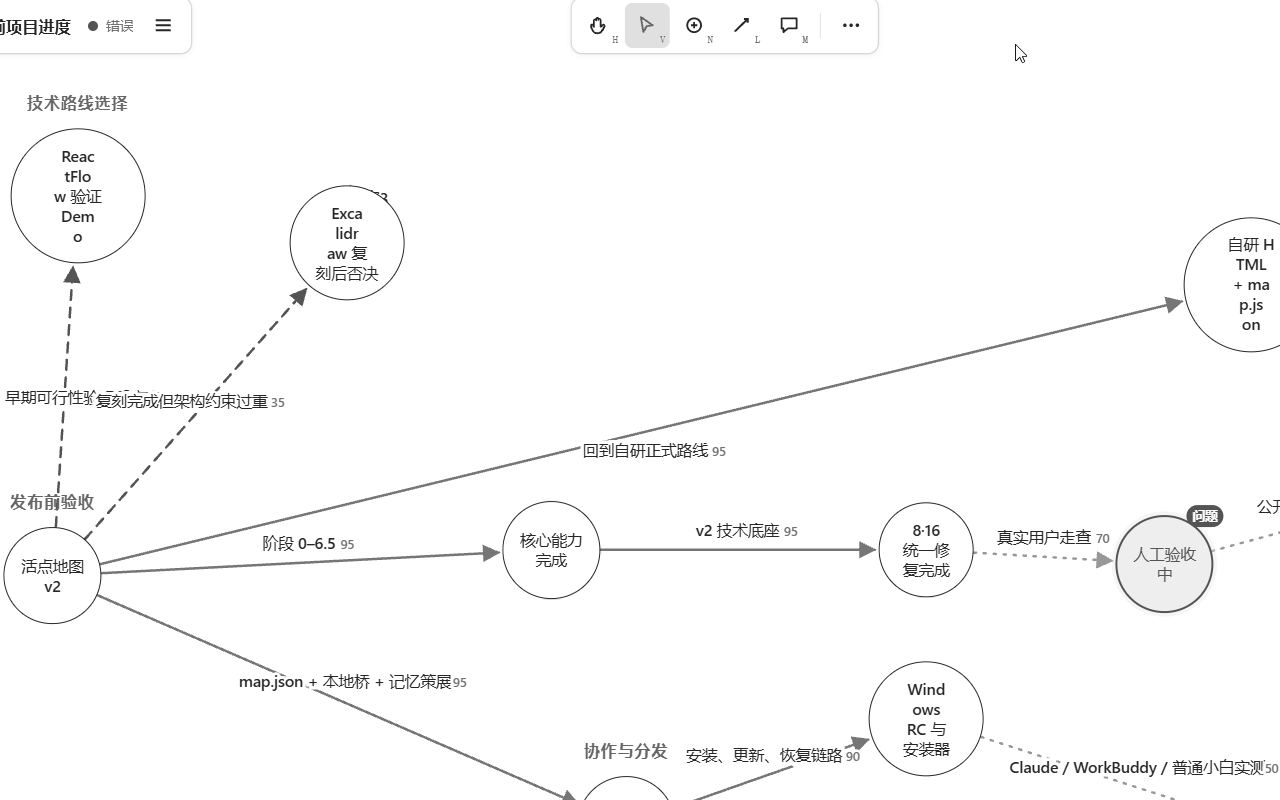
\includegraphics[width=0.96\textwidth,height=0.74\textheight,keepaspectratio]{images/fig6-project-memory-print.png}
\patentfigurelabel
\end{center}
\clearpage

\vspace*{1.0cm}
\begin{center}
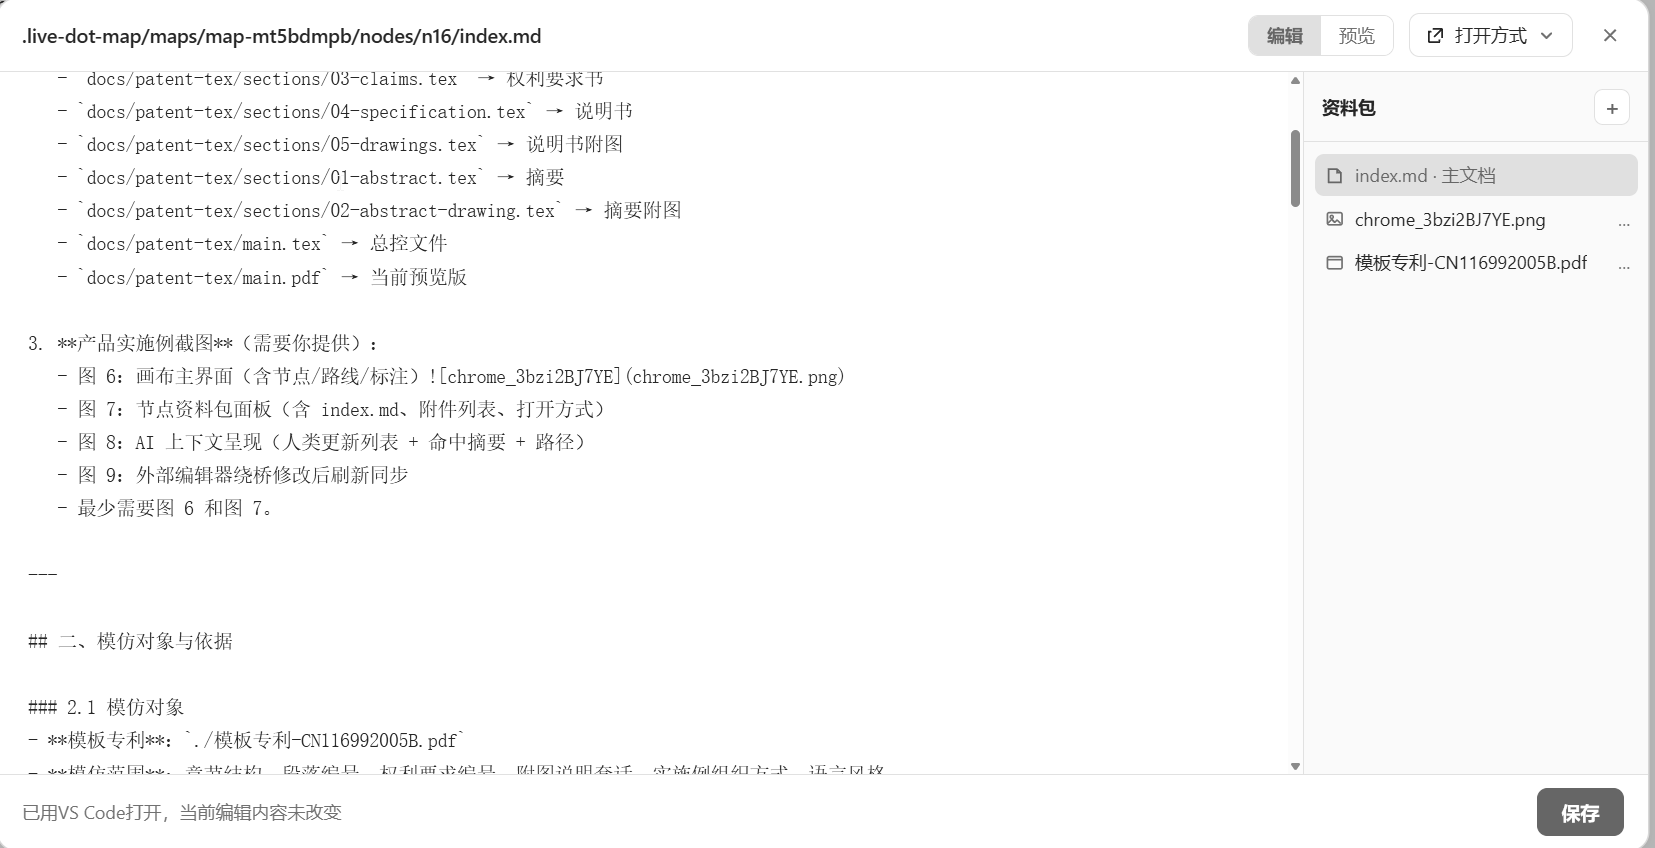
\includegraphics[width=0.96\textwidth,height=0.74\textheight,keepaspectratio]{images/fig7-bundle-print.png}
\patentfigurelabel
\end{center}
\clearpage

\vspace*{1.0cm}
\begin{center}
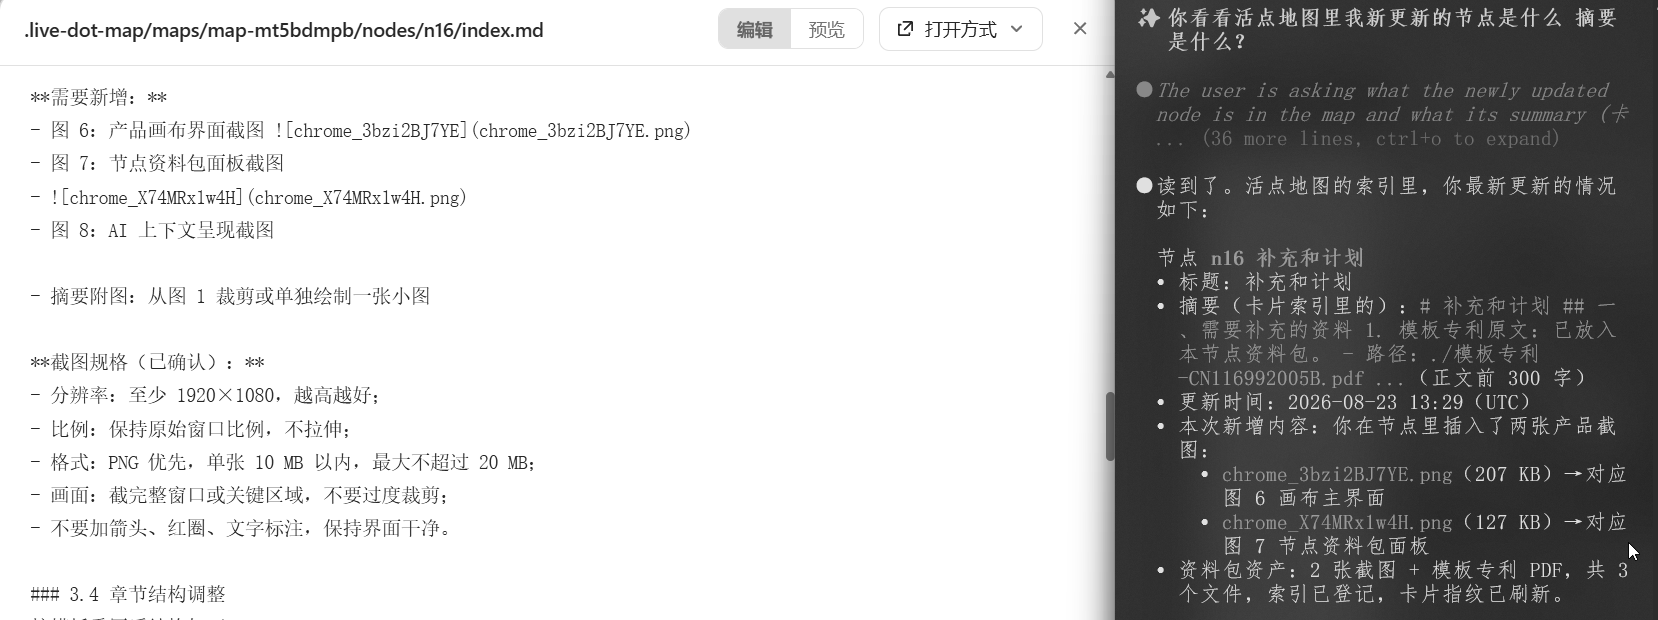
\includegraphics[width=0.96\textwidth,height=0.74\textheight,keepaspectratio]{images/fig8-agent-print.png}
\patentfigurelabel
\end{center}
